\chapter{Influence of phytoplankton-derived dissolved organic matter on marine bacterial community dynamics on the Western Antarctic Peninsula}\label{ch:dom}

\chapterdisclaimer{This work was performed in collaboration with Linda Amaral-Zettler, Hugh Ducklow, Daniel Repeta, Andrew Rhyne, and Jeremy Rich.\\
\\
Catherine Luria, Linda Amaral-Zettler, Hugh Ducklow, and Jeremy Rich designed and conducted the study with assistance from Dan Repeta and Andrew Rhyne. Linda Amaral-Zettler and Jeremy Rich contributed sequence data for the study. Catherine Luria analyzed data and wrote this chapter with guidance from Jeremy Rich. 
}


\section{Abstract}

Bacterial interactions with dissolved organic matter (DOM), largely produced by phytoplankton, drive much of the movement of carbon through the oceanic food web and the global carbon cycle. The extent to which DOM, especially phytoplankton exudates, drives bacterial community assembly is unclear and describing the complex interactions between bacteria and marine DOM remains an important challenge. The marine ecosystem of the Western Antarctic Peninsula (WAP) undergoes a dramatic seasonal transition each spring that culminates in intense summer phytoplankton blooms, providing a dynamic system in which to study these interactions. We tested the hypothesis that WAP bacterial growth and community succession are primarily driven by the availability of labile DOM  through a series of mesocosm experiments that spanned the WAP spring transitional period (August-December 2013). The addition of DOM, in the form of cell-free exudates extracted from \emph{Thalassiosira weissflogii} diatom cultures to 50-L mesocosms led to changes in bacterial abundance, production, and community composition. The timing of each experiment (i.e. early spring versus late spring) influenced the magnitude and direction of these changes. For example, the same DOM treatment applied at different times during the season resulted in different levels of bacterial production and different bacterial community composition, including a striking mid-season shift between Colwelliaceae and \emph{Polaribacter}. Our findings suggest that the timing of phytoplankton blooms can alter bacterial community response, perhaps indicating the influence of priority effects. Strong interannual variability as well as long-term climate change may shift the timing of WAP phytoplankton blooms and bacterial responses to this shift could have profound implications for the bacterial-mediated movement of carbon and nutrients through the WAP ecosystem.

\section{Introduction}

Marine dissolved organic matter (DOM) represents the largest exchangeable reservoir of carbon on Earth and drives a considerable fraction of the oceanic food web \citep{hedges1992global}. Phytoplankton production is the dominant source of marine organic material, with an estimated 50\% of algal production entering the DOM pool through a variety of mechanisms \citep{lampert1978release,fogg1983ecological,gobler1997release}. The resulting DOM pool is a complex mixture of thousands of organic compounds with varying degrees of lability. Over 90\% of the material released by algae is considered labile and is consumed and respired within days; meanwhile, a wide variety of more recalcitrant compounds accumulate in seawater and are available for long-term sequestration in the deep ocean \citep{ducklow2001seasonal}. Despite long-term ramifications for atmospheric \ce{CO_2} concentrations, the interplay between diverse bacterial assemblages and complex DOM pools is poorly understood. 

 

Phytoplankton blooms are associated with shifts in bacterial community composition \citep{Pinhassi2004-kc,Teeling2012-jz,Klindworth2014-ba}, perhaps due to changes in DOM availability and composition. Previous studies provide conflicting reports of generalist assemblages that can utilize a wide variety of substrates \citep{mou2007bacterioplankton,newton2010genome,chronopoulou2015generalist} as well as communities of specialists that are adapted to take advantage of only certain classes of DOM compounds and respond quickly to disturbance \citep{cottrell2000natural,am08,nelson2012tracking,sarmento2012use,Klindworth2014-ba,sharma2014distinct}. Nonetheless, some general trends based on broad taxonomic groups have emerged. For example, certain groups of bacteria (e.g., Flavobacteria and Rhodobacteraceae) tend to increase in abundance during phytoplankton blooms, while other groups such as \emph{Pelagibacter} appear better adapted to non-bloom conditions \citep{williams2013role,Buchan2014-yh,Voget2015-ch}. 

 

The Western Antarctic Peninsula (WAP) provides a dynamic environment in which to study bacterial response to phytoplankton blooms. The WAP system undergoes an extreme seasonal transition every spring, from almost total darkness to almost continuous sunlight, resulting in a synchronized cascade of environmental changes that culminates in intense phytoplankton blooms, supporting a highly productive food web \citep{Venables2013-me,Smetacek2005-tz}. Bacterioplankton activity closely follows the annual phytoplankton cycle and bacterial growth and succession are thought to be largely driven by DOM availability \citep{Kirchman2009-sg,dsvse12}, the relationship between phytoplankton-derived DOM and bacteria has not been directly tested. Furthermore, the WAP is subject to strong inter-annual variability in sea ice and upper water column dynamics, while dramatic warming of the WAP region over the last 50 years has reduced sea ice extent and led to earlier sea ice retreat in the spring \citep{saba2014winter,vaughan1996recent,mk05,thomas2009ice,Stammerjohn2008-nj}. It is not known how changes in the timing of sea ice retreat, and subsequently of phytoplankton blooms, may alter bacteria-DOM interactions and carbon cycling. 

We conducted a series of DOM-addition mesocosm experiments that spanned the WAP spring transitional period to examine how pre-bloom communities react to changes in DOM availability. While many previous DOM-addition experiments have relied upon relatively simple compounds (e.g. glucose or amino acids), which may be poor analogs for the organic carbon utilized by marine bacteria in the WAP \citep{dmegm11,straza2010abundance}, we used diatom exudates, a more complex substrate. Our goals were to assess how diatom exudates alter the bacterial community and how these alterations change depending on the timing of the experiment in relation to the season. We hypothesized that DOM additions would change bacterial community composition and that the magnitude of these DOM-driven changes would decrease as the season progressed and organic carbon availability increased in the environment. 

 

\section{Methods}

\subsection{DOM preparation} 

Large-scale (500L) axenic cultures of \emph{Thalassiosira weissflogii}, a well-characterized marine diatom, were grown in f/2 medium \citep{f2guillard1975} in custom acid-washed polycarbonate containers. The cultures were harvested at seven days when they had developed dense growth but were still in the exponential growth phase. Previous work shows that \emph{T. weissflogii} DOM exudates collected at this stage are primarily comprised of carbohydrates, acetate, and lipids and are enriched for carbohydrates relative to seawater \citep{aluwihare1999comparison}. The create an f/2 "control," the same volume of f/2 media was treated identically, but was not inoculated with \emph{T. weissflogii}. This control was to account for any DOM in the f/2 seawater itself. 

Cells and particulate matter were removed via peristaltic pump-driven serial filtration through combusted GF/F filters (Whatman, GE Healthcare Life Sciences, Piscataway, NJ, USA) and acid-washed \SI{0.2}{\micro\meter} polyethersulfone membrane filter capsules (Whatman, GE Healthcare Life Sciences, Piscataway, NJ, USA) using acid-washed platinum-cured silicon tubing (Masteflex, Cole Parmer, Vernon Hills, IL). The filtrate was collected in clean acid-washed polycarbonate containers, acidified by adding sufficient hydrochloric acid to lower the pH to \textasciitilde{}5.0, and stored in the dark until further processing. 

Solid phase extraction of DOM, which has been shown to capture \textasciitilde{}60\% of marine DOM on average \citep{dittmar2008simple}, was performed by pumping the filtrate through C18 HPLC columns (Cole Parmer, Vernon Hills, IL) at a rate of 50 ml min$^{-1}$. The columns were prepared by gravity-driven flushing with 100 ml methanol followed by 200 ml of MilliQ water (EMD Millipore, Merck KGaA, Darmstadt, Germany). DOM was eluted from the C18 columns into combusted roundbottom flasks by flushing the columns with 100 ml of methanol. The DOM solution was gently warmed to 35 \textdegree C and was concentrated by vacuum evaporation followed by flushing with nitrogen gas as needed, leaving a dried residue suitable for transport. Aliquots of the DOM solution were retained to measure DOC concentration on a Shimadzu TOC analyzer (Shimadzu, Inc., Columbia, MD). 

Prior to mesocosm experiments, the dried DOM was re-dissolved in a \SI{0.2}{\micro\meter}-filtered 10 mM sodium hydroxide solution. The solution was centrifuged for 15 minutes at 3240 rpm to remove any particulate matter, which was retained, dried, and weighed to re-calculate the DOC concentration and make necessary amendment volume adjustments. 

 

\subsection{Mesocosm experiments}

Mesocosm experiments were conducted in August, September, October, and December 2013 at Palmer Station, Antarctica. Acid-washed 50 L polycarbonate carboys were filled directly from a seawater intake located at a depth of 6 m, 16 m from the shore. The intake was sampled prior to any filtering on station. The collected water was divided into two groups: (1) control (no additions, $n=3$) and (2) +DOM (\SI{40}{\micro\mole} DOM addition; $n=3$). An additional f/2 control treatment ($n=3$) was included in the October experiment. The carboys were incubated for 10 days under \emph{in situ} temperatures and continuous light with PAR levels inside the carboys of \SI{1e15}{quanta~\cm^{-2}~\second^{-1}} inside carboys).

Chlorophyll \emph{a} (chl \emph{a}) and phaeopigment, dissolved organic carbon (DOC), dissolved inorganic nutrients (phosphate, silicate, nitrite and nitrate), and bacterial production ($^{3}$H-leucine incorporation rates) were assessed every 48 hours for 10 days using methods previously described in Chapter 3. Bacterial abundance samples were also collected every 48 hours and were analyzed by flow cytometry with SYBR \textsuperscript{\textregistered} Green I nucleic acid staining (Invitrogen, Carlsbad, CA) on a Guava easyCyte flow cytometer (EMD Millipore, Billerica, MA). Samples for bacterial community composition were collected on days 0, 6, and 10 by filtering \textasciitilde{}2L water through successive \SI{3.0}{\micro\meter} polycarbonate and \SI{0.22}{\micro\meter} polyethersulfone (EMD Millipore, Billerica, MA) filters. Filters were flash-frozen with liquid \ce{N_2} and stored at -80\textdegree C until further processing. Samples for particulate organic carbon (POC) and particulate organic nitrogen (PON) were collected on days 0 and 10 as described in Chapter 3. All sampling took place at incubation temperatures. 

 

\subsection{16S rRNA gene library generation} 

Sequence libraries were generated as in \citet{Eren2013-ob}, with modifications as described in Chapter 3. Briefly, DNA was extracted from cells captured on the \SI{0.22}{\micro\meter} pore size filters (i.e. "free-living" bacterioplankton) using a DNeasy Plant Mini Kit (Qiagen, Valencia CA) with an additional bead-beating step. For each DNA sample, the V6 hypervariable region of the 16S rRNA gene was amplified by polymerase chain reaction (PCR) with custom fusion primers that contained Illumina adaptors and inline barcodes (forward primer) or dedicated indices (reverse primer) \citep{Eren2013-ob}. Size-selected PCR products were quantified and pooled in equimolar amounts prior to sequencing on one lane of an Illumina HiSeq 1000 cycle paired-end run. 

Low-quality sequences were filtered from the resulting data by discarding reads without 100\% consensus between forward and reverse paired-end sequencing reads \citep{Eren2013-ob}, resulting in more than 16 millions sequences across 81 libraries. OTUs were clustered using Qiime (v 1.9.1; \citealt{Caporaso2010-ee}) with open reference OTU picking with the default UCLUST method (Edgar 2010), a minimum cluster size of 2, and a 97\% similarity threshold and were assigned Greengenes taxonomy (version 13\_8; \citealt{McDonald2012-qf}). After removing OTUs classified as Chloroplasts, rarefied libraries were produced by randomly down-sampling to the smallest library size of 64271 sequences spread among 14751 OTUs. All of our sequence data are MIMARKS-compliant \citep{Yilmaz:2011aa} and will be deposited in the NCBI Sequence Read Archive. 

\subsection{Data analysis}

We estimated community turnover rate by dividing carbon biomass, derived from bacterial abundance with a conversion factor of \SI{e-14}{\gram} C per cell, by the rate of carbon uptake, derived from bacterial production measurements with a conversion factor of 1500 g C per mole \ce{^3H}-leucine incorporated. To separate the effects of experiment month, experiment day (i.e. days into incubation period), and treatment on environmental parameters, we used ANOVA to compare linear models based on different combinations of independent variables using the \code{lm} and \code{anova} functions in R \citep{t08}. 

Alpha diversity metrics, including the number of OTUs observed in each library, Shannon's diversity, and Pielou's evenness, were calculated using the \code{BiodiversityR} package in R \citep{kindt2005tree}. The beta diversity between samples was visualized with non-metric multidimensional scaling (NMDS) based on Bray-Curtis similarity using the \code{metaMDS} function in the \code{vegan} R package \citep{Oksanen_2015}. Co-occurrence network analyses based on Pearson's correlations revealed relationships among OTUs and between OTUs and external variables (i.e. experimental treatments and bacterial production). Networks were generated using the Cytoscape CoNet plugin (version 1.1.1.beta; \citealt{faust2012microbial}) and were visualized in Cytoscape (version 3.4.0; \citealt{smobwr}). Copies of the MIMARKS table and chapter figures as well as the R code used for all data analysis and figure production can be accessed at: \url{https://github.com/cmluria/dissertation/Chapter_4_DOM}. 

\section{Results}

Our experiments spanned the winter-to-late spring period, which was characterized by relatively consistent environmental conditions before the onset of an intense phytoplankton bloom in January, described in Chapter 3. Chl \emph{a} remained quite low, below \SI{1}{\micro\gram \per\liter} in the environment except for brief increase to \SI{2.8}{\micro\gram \per\liter} that corresponded to the onset of our October experiment, compared to a peak in chl \emph{a} of \textasciitilde{}\SI{20}{\micro\gram \per\liter} during the summer bloom (Figure \ref{fig:ch3:swi}  and \ref{fig:ch3:chla_poc_pon} ). During our experimental period (August - December 2013), temperatures increased steadily from -1.2 to 0.8\textdegree C. Sea ice persisted into December, beyond our last experiment, and water column light availability would have been relatively low \citep{massom2014state}. Inorganic nutrients (nitrate and nitrite, phosphate, silicate) were somewhat lower in October, corresponding to the brief increase in chl \emph{a}, but were never depleted (Figure \ref{fig:ch3:swi}  and \ref{fig:ch3:nutrients} ). DOC increased from \textasciitilde{}\SI{40}{\micro\mole} in August to \textasciitilde{}\SI{60}{\micro\mole}  in December. POC increased from \textasciitilde{}\SI{10}{\micro\gram \per\liter}  at the onset of the first experiment to \textasciitilde{}\SI{70}{\micro\gram \per\liter}  at the onset of the last experiment, but this increase is minor relative to the \SI{800}{\micro\gram \per\liter}  recorded during the January phytoplankton bloom. There was a slight enrichment of POC at the beginning of the experiments in DOM+ mesocosms, corresponding to \textasciitilde{}10\% of added DOC (Figure \ref{fig:ch3:swi}  and \ref{fig:ch3:chla_poc_pon}). While bacterial abundance was fairly stable, bacterial production increased slightly, from {\textless}\SI{1}{\pico\mole \per\liter \per\hour} to \textasciitilde{}\SI{5}{\pico\mole \per\liter \per\hour}  during the experimental period, compared to a peak of \textasciitilde{}\SI{120}{\pico\mole \per\liter \per\hour}  during the January bloom (Figure \ref{fig:ch3:environment_BA_BP_turnover}). This increase was associated with a doubling of the community turnover rate (Figure \ref{fig:ch3:environment_BA_BP_turnover}). 

\begin{figure}[htbp] 
\centering 
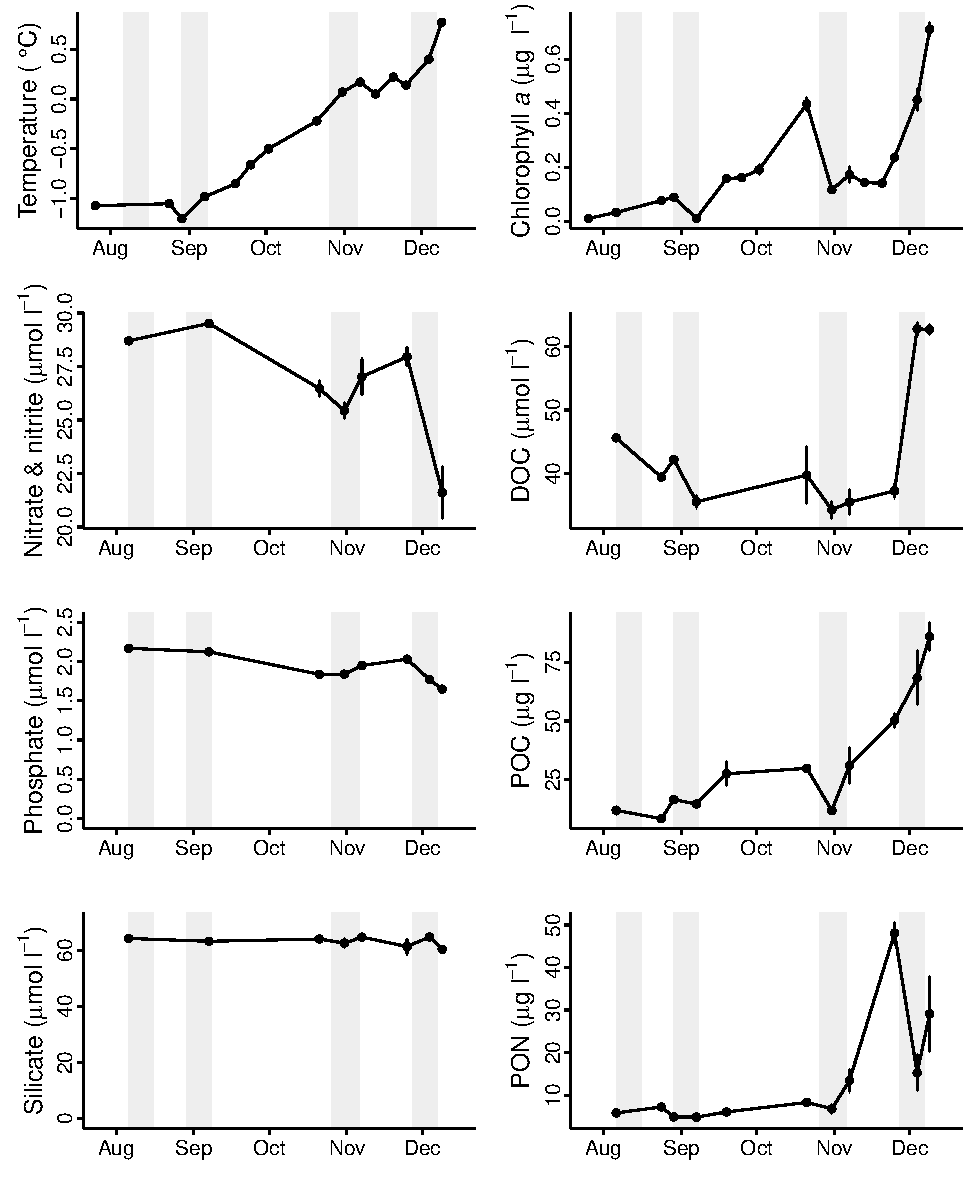
\includegraphics[width=0.8\textwidth]{Chapter_4_DOM/Figures/Supplemental_Figure_1_SWI_data}
\caption[Environmental conditions during the experimental period, August-December 2013.]{Temperature, inorganic nutrients (nitrate/nitrite, phosphate, silicate), chlorophyll \emph{a}, DOC, POC, and PON in the environment during the experimental period, August – December 2013. The timing of the four experiments is indicated by shaded bars.} 
\label{fig:ch3:swi} 
\end{figure}

\begin{figure}[ht!] 
\centering 
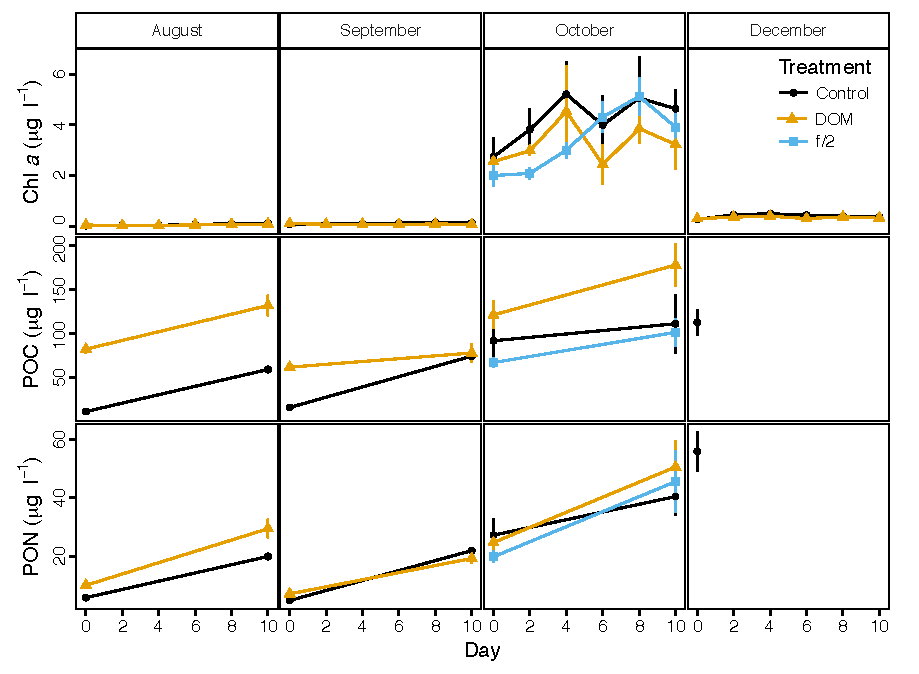
\includegraphics[width=\textwidth]{Chapter_4_DOM/Figures/Supplemental_Figure_2_Chla_POC_PON}
\caption[Chlorophyll \emph{a}, particulate organic carbon, and particulate organic nitrogen concentrations over the course of four experiments.]{Chlorophyll \emph{a}, particulate organic carbon, and particulate organic nitrogen concentrations over the course of four experiments.
} 
\label{fig:ch3:chla_poc_pon} 
\end{figure}

\begin{figure}[ht!] 
\centering 
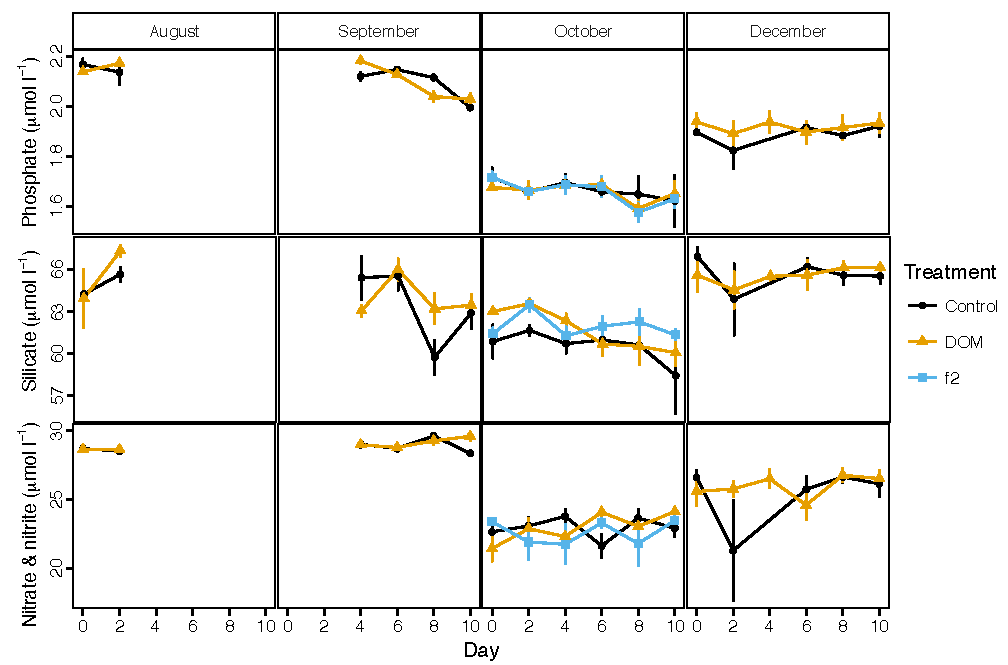
\includegraphics[width=\textwidth]{Chapter_4_DOM/Figures/Supplemental_Figure_3_Nutrients}
\caption[Inorganic nutrient (phosphate, silicate, and nitrate/nitrite) concentrations over the course of four experiments.]{Inorganic nutrient (phosphate, silicate, and nitrate/nitrite) concentrations over the course of four experiments.} 
\label{fig:ch3:nutrients} 
\end{figure}

\begin{figure}[ht!] 
\centering 
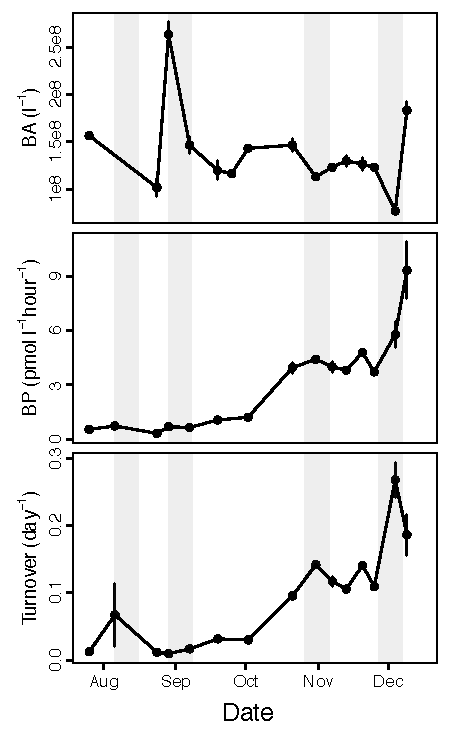
\includegraphics[width=0.5\textwidth]{Chapter_4_DOM/Figures/Figure_1_environment_BA_BP_turnover}
\caption[Bacterial abundance, bacterial production, and estimated community turnover rates in the environment during the experimental period, August – December 2013.]{Bacterial abundance (BA), bacterial production (BP), and estimated community turnover rates in the environment during the experimental period, August – December 2013. The timing of the four experiments is indicated by shaded bars.} 
\label{fig:ch3:environment_BA_BP_turnover} 
\end{figure}


Bacterial abundance increased over time in both control and DOM+ mesocosms, but the increases were more substantial in the DOM+ mesocosms than in the control mesocosms after Day 6 of the August, September, and October experiments (Figure \ref{fig:ch3:BA_BP_Turnover_Richness}). Although the initial values were similar, final DOM+ cell abundances were \textasciitilde{}50\% greater in October than in August and September. Treatment ($p = 0.0002$) and incubation day ($p = 6 \times 10^{-12}$) were more important drivers of variability than month ($p = 0.01$). Bacterial production (BP) increased over time in all mesocosms, but there were differences in BP between control and DOM+ mesocosms (Figure \ref{fig:ch3:BA_BP_Turnover_Richness}). During the first part of the season (August and September), BP increased more quickly in the DOM+ mesocosms, but BP in the control mesocosms ultimately reached similar levels, with 200- to 400-fold increases in all mesocosms. In the later part of the season (October and December) BP was fairly stable in the control mesocosms, with only 2- to 3-fold increases by Day 10. BP increased in the DOM+ mesocosms, but did not reach the same levels as earlier in the season, with only 10- to 20-fold increases. While BP varied between control and DOM+ mesocosms, treatment effects were less significant ($p < 0.005$) than the effects of day and month (both $p < 10^{-6}$). Estimated turnover rates tracked bacterial production, with the highest rates occurring in the DOM+ mesocosms in the August and September experiments.


\begin{figure}[ht!] 
\centering 
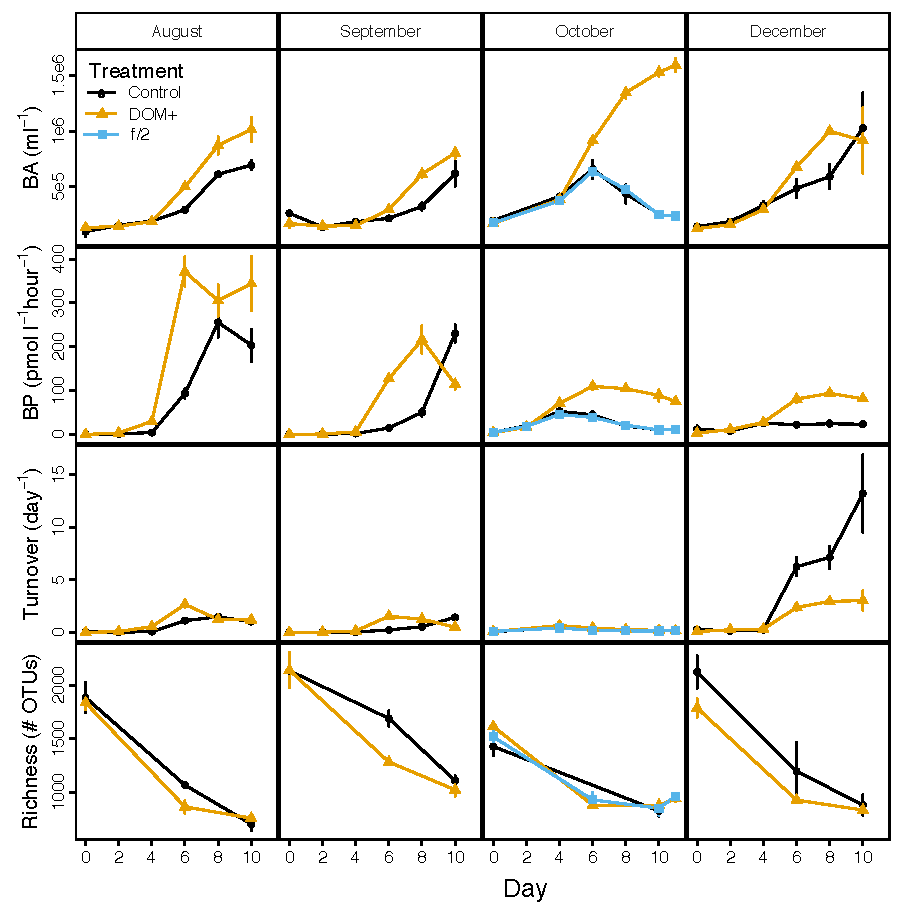
\includegraphics[width=0.9\textwidth]{Chapter_4_DOM/Figures/Figure_2_BA_BP_Turnover_Richness}
\caption[Bacterial abundance, bacterial production, estimated community turnover rates, and OTU richness over the course of four experiments.]{Bacterial abundance (BA), bacterial production (BP), estimated community turnover rates based on abundance and production, and observed OTU richness over the course of four experiments.} 
\label{fig:ch3:BA_BP_Turnover_Richness} 
\end{figure}


OTU richness, which was around 2000 OTUs on Day 0 of the August, September, and December experiments, had dropped to {\textless}1000 OTUs by Day 10 (Figure \ref{fig:ch3:BA_BP_Turnover_Richness}). Day 0 richness was slightly lower (\textasciitilde{}1500 OTUs) during the October experiment, but reached Day 10 levels similar to those in the other experiments. Evenness and Shannon diversity also declined in most mesocosms (Figure \ref{fig:ch3:alpha_diversity}). As with bacterial production, although the rate of decline sometimes varied between control and DOM+ mesocosms, day ($p < 2 \times 10^{-16}$) and month ($p < 10^{-6}$) outweighed treatment effects ($p < 0.1$). While OTU richness was significantly negatively correlated with both bacterial production ($p = 10^{-6}, r^{2}=0.25$) and abundance ($p < 3 \times 10^{-8}, r^{2}=0.35$), experimental day alone explained that greatest amount of variance ($r^{2}=0.71, p < 2 \times 10^{-16}$). 

\begin{figure}[htbp] 
\centering 
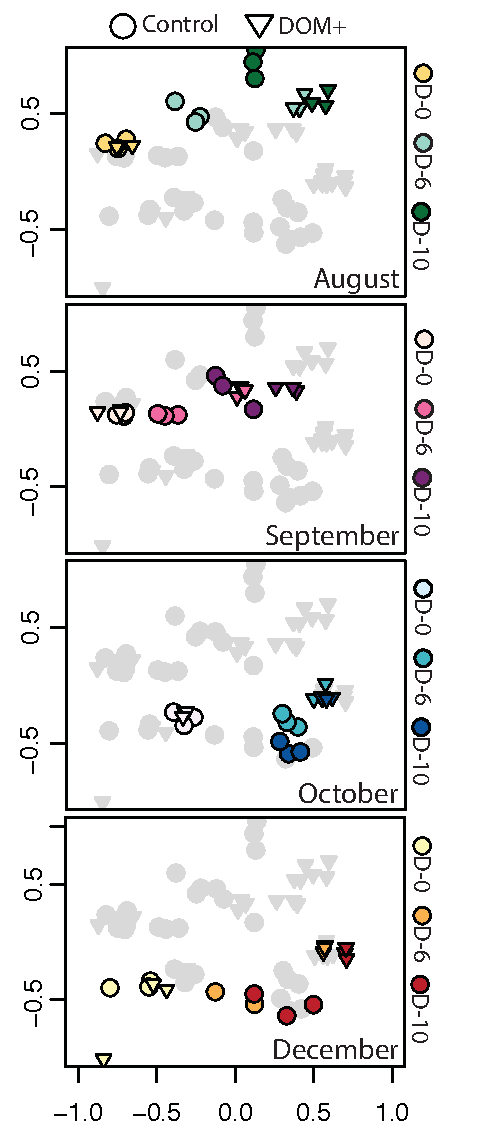
\includegraphics[width=0.5\textwidth]{Chapter_4_DOM/Figures/Figure_3_nmds}
\caption[Non-metric multidimensional scaling (NMDS) of Bray-Curtis similarity indices based on OTU relative abundance.]{Non-metric multidimensional scaling (NMDS) of Bray-Curtis similarity indices based on OTU relative abundance. Each point corresponds to an individual mesocosm replicate and sampling date ($n=3$ per time point per treatment). All samples from all experiments are shown in each panel. A different experiment is highlighted in each panel, with all other experiments shown in grey. Within each panel, different colors correspond to different sample days (0, 6, and 10). Control mesocosm communities are denoted by circles and DOM+ mescosm communities are denoted by triangles. For day 6 of the October experiment, f/2 control data is show in lieu of the regular control.} 
\label{fig:ch3:nmds} 
\end{figure}

\begin{figure}[ht!] 
\centering 
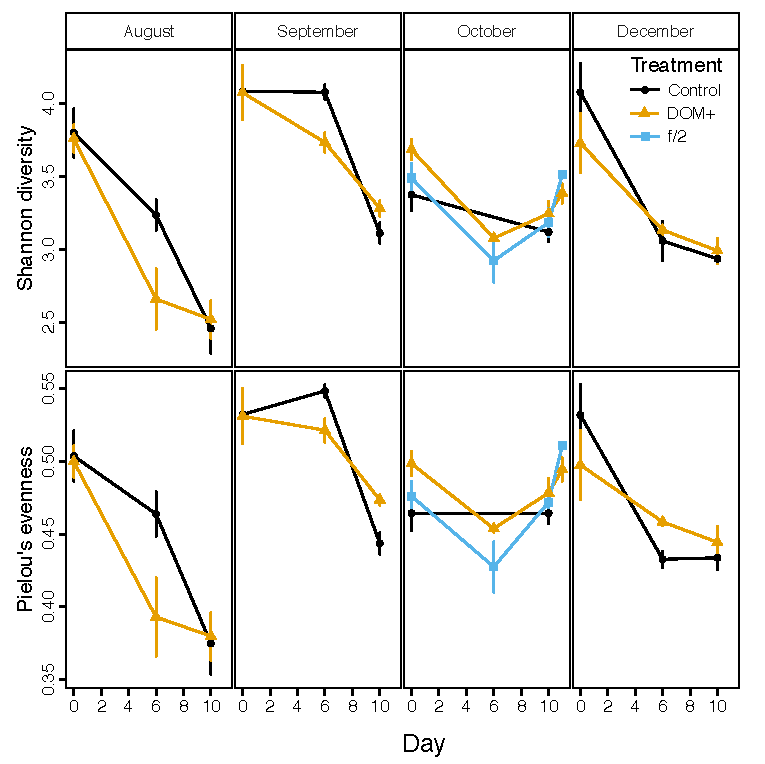
\includegraphics[width=\textwidth]{Chapter_4_DOM/Figures/Supplemental_Figure_4_alpha_diversity}
\caption[Alpha diversity metrics (Shannon diversity and Pielou’s evenness) over the course of four experiments.]{Alpha diversity metrics (Shannon diversity and Pielou’s evenness) over the course of four experiments.} 
\label{fig:ch3:alpha_diversity} 
\end{figure}

NMDS based on Bray-Curtis similarity visualizes how communities changed between months, experimental time points, and treatments (Figure \ref{fig:ch3:nmds}). NMDS axis 1 reflects changes that occurred within each experiment. By Day 6, the DOM+ mesocosm communities had reached or were quite close to their Day 10 state, while the control mesocosm communities continued to change as the experiment progressed. NMDS axis 2 reflects changes between experiments. The early spring experiments (August and September) and late spring experiments (October and December) are closely aligned with each other, but a relatively large shift occurred between September and October. Community composition in the first pair of experiments remained distinct from that in the second pair of experiments through the whole incubation period, indicating that the starting community composition was an important factor influencing the final community composition.


\begin{figure}[ht!] 
\centering 
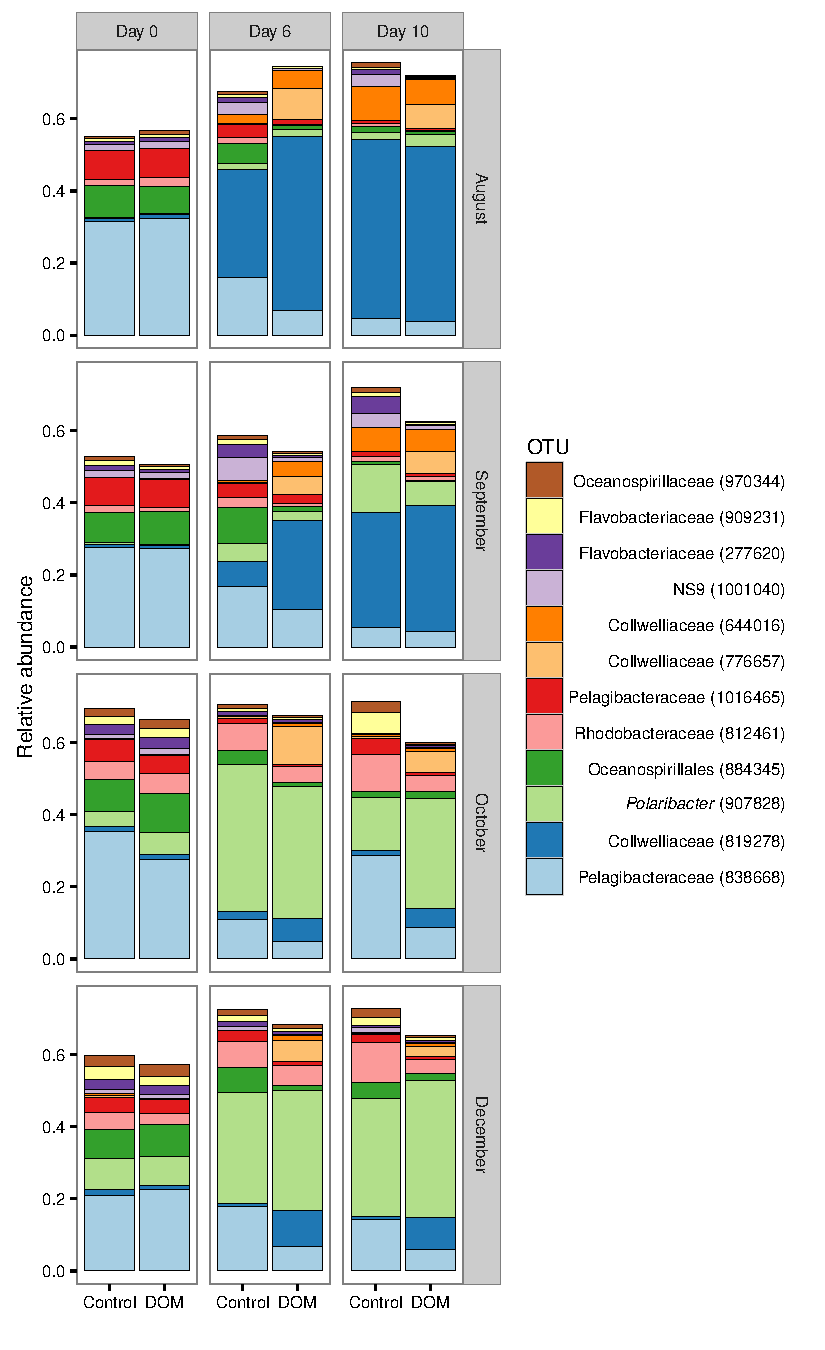
\includegraphics[width=0.8\textwidth]{Chapter_4_DOM/Figures/Figure_4_OTU_barplot}
\caption[Changes in the mean relative abundance of the top 12 OTUs (by mean relative abundance) across all experiments.]{Changes in the mean relative abundance of the top 12 OTUs (by mean relative abundance) across all samples. On Day 6 of the October experiment, the f/2 control is shown in lieu of the regular control.} 
\label{fig:ch3:otu_barplot} 
\end{figure}


Figure \ref{fig:ch3:otu_barplot}  shows the relative abundances of the top 12 OTUs (by mean relative abundance across all samples), which together represent ~50-75\% of each community. In all four experiments, OTUs classified as Pelagibacteraceae, Oceanospirillales, and SAR324 declined over time, while OTUs classified as Collwelliaceae and \emph{Polaribacter} increased in relative abundance. However, the relative importance of the two most abundant OTUs, Collwelliaceae (819278) and \emph{Polaribacter} (907828), shifted between September and October, with relatively small changes in initial community composition between September and October corresponding to much larger differences by the end of each experiment (Figure \ref{fig:ch3:otu_barplot}). In August and September, Collwelliaceae was slightly more abundant than \emph{Polaribacter} at Day 0. By Day 10, this difference was exaggerated with Collwelliaceae making up \textasciitilde{}40\% while \emph{Polaribacter} made up only \textasciitilde{}20\% of the community. As the season progressed, \emph{Polaribacter} became more prominent in the environment and the trend during experiments was reversed; by the end of the October and December experiments, Collwelliaceae made up only \textasciitilde{}7\% of the community, while Polaribacter made up \textasciitilde{}35\% of the community in DOM+ mesocosms. Of the top 12 OTUs, 6 varied in relative abundance by 5\% or more at one or more time points between the DOM+ and control communities (Figure \ref{fig:ch3:treatment_effect}). Colwelliaceae (819278 and 776657) were always more abundant in the DOM+ mesocosms, while Rhodobacteraceae (812461), Oceanospirillales (884345), and Pelagibacteraceae (838668) were always more abundant in the control. \emph{Polaribacter} (907828) displayed both positive and negative treatment effects at different times. 

\begin{figure}[htbp] 
\centering 
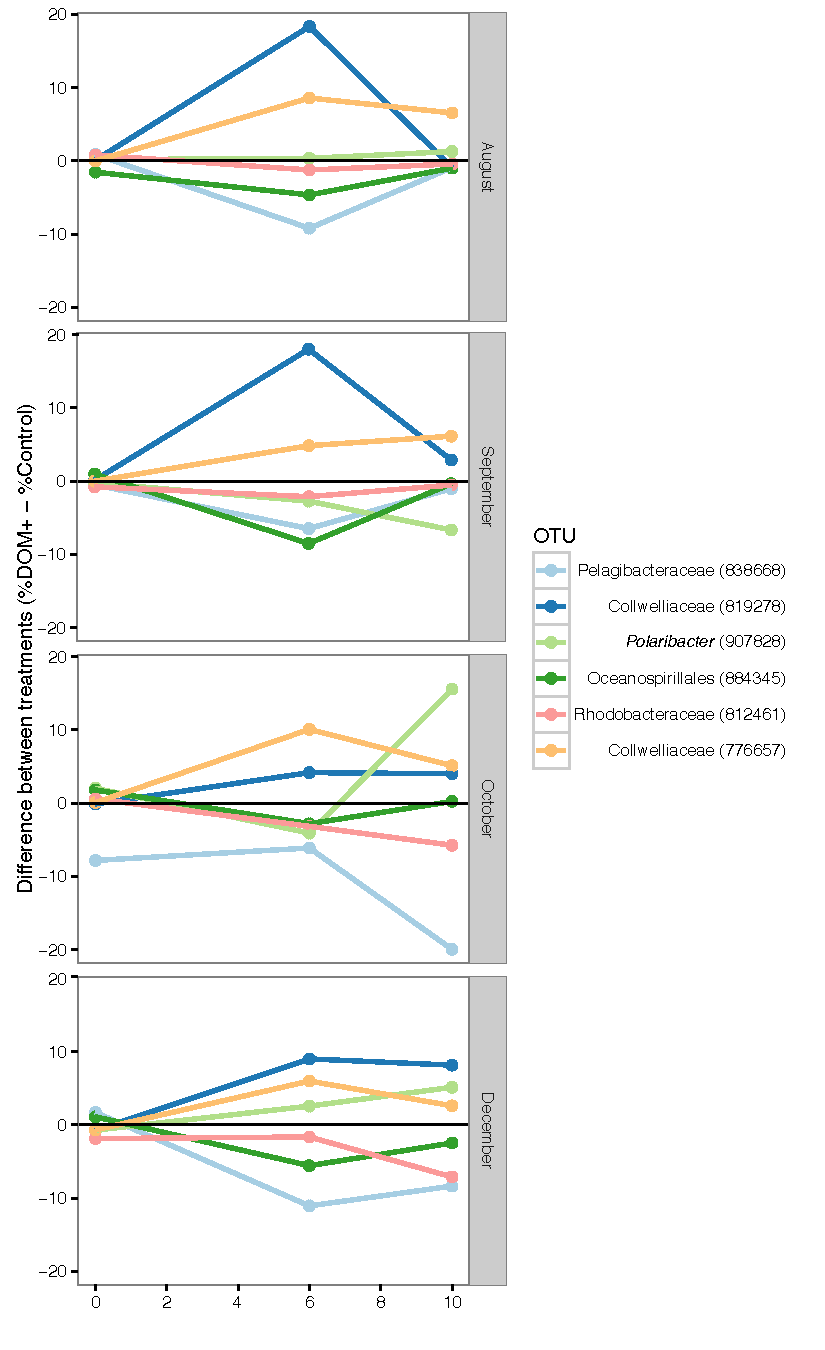
\includegraphics[width=0.8\textwidth]{Chapter_4_DOM/Figures/Figure_5_treatment_effect}
\caption[Difference in OTU relative abundance (\%) between the DOM-amended and control mesocosms.]{Difference in OTU relative abundance (\%) between the DOM-amended and control mesocosms. Out of top 12 OTUs (by mean relative abundance, see Figure 2), only OTUs showing more than ±5\% change are plotted. On Day 6 of the October experiment, the f/2 control is shown in lieu of the regular control.} 
\label{fig:ch3:treatment_effect} 
\end{figure}

We identified a sub-network of OTUs that were significantly associated with either the control group or the DOM treatment ($r > 0.5$; Figure \ref{fig:ch3:network}). All of the OTUs that were positively correlated with DOM+ were classified as Gammaproteobacteria, primarily Colwelliaceae. Several, but not all of these OTUs were negatively correlated with the control. Only one OTU, classified as NS9, was positively correlated with the control. A second sub-network linking OTUs to bacterial production shows that many Colwelliaceae OTUs correlated positively with bacterial production, as opposed to a number of Alphaproteobacteria OTUs, over half of them classified as Pelagibacteraceae, as well as two Gammaproteobacteria, HTCC2089 and HTCC2188, which were negatively correlated ($r > 0.7$).

\begin{figure}[htbp] 
\centering 
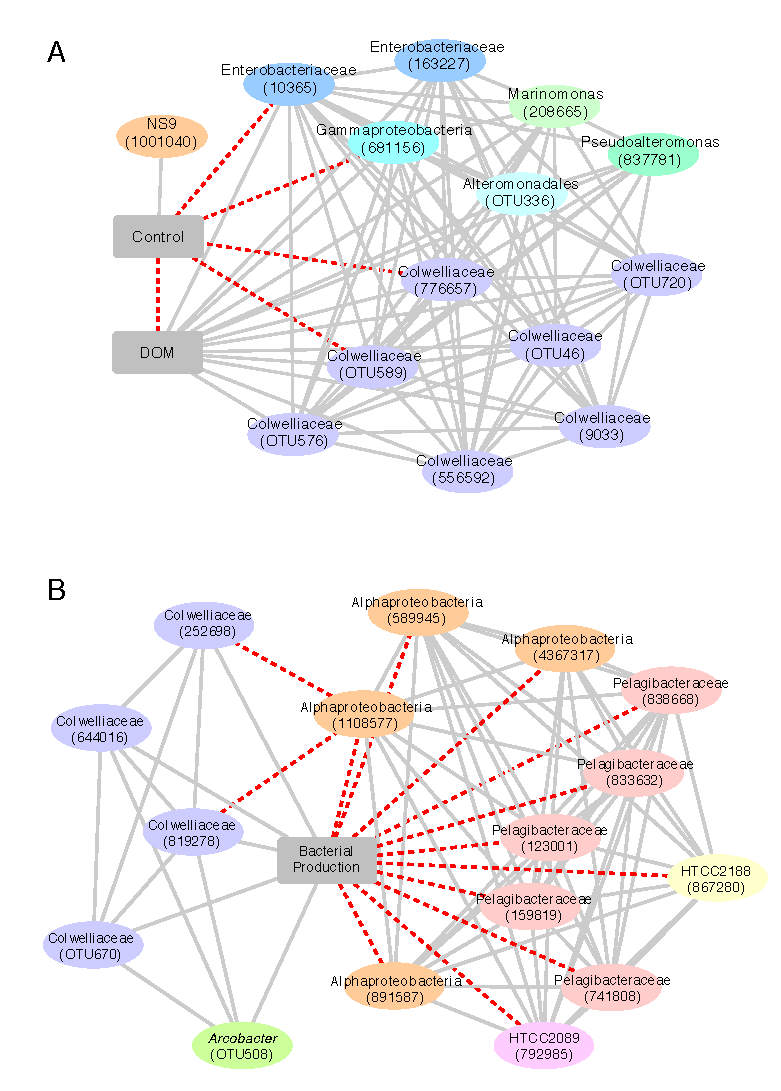
\includegraphics[width=0.9\textwidth]{Chapter_4_DOM/Figures/Figure_6_Network}
\caption[Sub-networks of highly correlated OTUs built around treatment level (control versus DOM+ and bacterial production.]{Sub-networks of highly correlated OTUs built around A) treatment level (control versus DOM+; $r > 0.5$) and B) bacterial production ($r > 0.7$). For clarity, only OTUs that appeared in at least 20\% of samples and had a mean relative abundance > $1$x$10^{-4}$ are shown. Solid, grey lines represent positive correlations; dashed, red lines represent negative correlations. Closest taxonomic identification and reference number (in parentheses) are given for each OTU.} 
\label{fig:ch3:network} 
\end{figure}

\section{Discussion}

Phytoplankton blooms and the resulting release of labile DOM are thought to be a major driver of marine bacterial community composition. Observational studies have shown that bacterial community composition and activity vary during phytoplankton blooms \citep{pinhassi2000seasonal,fandino2001variation,West2008-vp,tada2011differing,Teeling2012-jz,Klindworth2014-ba,wemheuer2015green}. This body of work suggests that bacterial succession allows for optimal DOM degradation, as bacterial groups with different metabolic strategies and substrate preferences display a high degree of niche partitioning in order to carry out different stages of DOM decomposition \citep{cottrell2000natural,alonso2007seasonal,poretsky2010transporter,rinta2012bacterial,sarmento2012use,Teeling2012-jz}. Niche partitioning may relieve direct competition between taxa and help explain high microbial diversity \citep{Teeling2012-jz,hutchinson1957concluding}. Alternatively, some studies have found that changes in DOM supply only slightly affect bacterial community composition, suggesting that physiological responses of metabolically versatile bacteria may be a factor, in addition to niche partitioning \citep{kirchman2004changes,rooney2005links,rink2007effects}.

There is growing evidence that labile organic matter availability is a primary factor controlling bacterial growth and community composition in Antarctica \citep{thingstad1991bacteria,Kirchman2009-sg,dsvse12,Kim2014-oj,luria2016seasonal}. However, directly testing the effects of phytoplankton-derived DOM on bacterial seasonal succession has proven challenging. Mesocosm experiments, like the one we conducted here, have traditionally relied on adding low molecular weight compounds like glucose or amino acids \citep{havskum2003silicate,allers2007response,gomez2012structuring}. For example, \citet{dmegm11} demonstrated that glucose enrichment of WAP seawater reduced bacterial diversity. Using more complex DOM substrates derived from phytoplankton cultures, several recent studies have shown that a wider range of bacteria respond readily to phytoplankton-, especially diatom-derived DOM, and that DOM originating from different phytoplankton species stimulates different bacterial phylogenetic groups \citep{sarmento2012use,nelson2012tracking,romera2011net}. Conversely, \citet{Landa2014-yg} and \citet{sharma2014distinct} found that varied natural DOM sources did not have differential effects on bacterial community composition despite variation in carbon quality and quantity. We selected the diatom \emph{T. weissflogii} as a DOM source as it is robust, well characterized, and a member of a genus that is widespread in the WAP region. However, the quantity and quality of DOM exuded by phytoplankton vary with species and physiological state and DOM from a single source (one species in one growth phase) does not represent the entire spectrum of changes in DOM composition and supply that probably occur during a phytoplankton bloom \citep{becker2014closely,Landa2014-yg}. 

Two OTUs were dominant across treatments, Colwelliaceae (819278) in the August and September experiments and \emph{Polaribacter} (907828) in the October and December experiments. Although marine Flavobacteria, including \emph{Polaribacter}, are heterotrophs that target high molecular weight organic matter and have been shown to increase in abundance during phytoplankton blooms, \emph{Polaribacter} did not show a consistent response to DOM amendments as opposed to simple `container effects,' the disturbance inherent in establishing a mesocosm \citep{cottrell2000natural,Pinhassi2004-kc,Abell2005-xu,gonzalez2008genome,Fernandez-Gomez2013-wr,Xing2015-kz,delong1993phylogenetic,Glockner1999-yc,West2008-vp,Teeling2012-jz}. The Colwelliceae family, on the other hand, responded quite strongly to DOM amendments, in excess of container effects. Colwelliaceae were abundant and diverse during the experiments, accounting for 9\% of all OTUs and 21\% of all sequences, as opposed to 3.6\% of OTUs and 2.6\% of sequences in the environment. A network of OTUs associated with DOM amendments was entirely comprised of Colwelliaceae and other Gammaproteobacteria. \emph{Colwellia} species are ubiquitous in polar environments and have been shown to metabolize an array of carbohydrates \citep{techtmann2016colwellia}. Interestingly, while Flavobacteria are perhaps more commonly associated with phytoplankton blooms, several previous studies have shown that Gammaproteobacteria, especially \emph{Alteromonas}, respond readily to natural DOM amendments during mesocosm experiments \citep{mccarren2010microbial,Landa2014-yg,romera2011net}.

Some of the changes in community structure observed during our experiments mirrored the changes that occur in the environment during a phytoplankton bloom. We compared abundant bacterial taxa from our mesocosm experiments to the seasonal time-series described in Chapter 3. Prevalent OTUs classified as Pelagibacteraceae (1016465 and 838668), Oceanospirillales (884345), and SAR324 (837879) decreased in both the experiment and the environment, while OTUs classified as \emph{Polaribacter} (907828), Flavobacteriaceae (1023473 and 909231), and Rhodobacteraceae (812461 and 789131) increased in both. Some of these changes presumably reflect resource partitioning to allow for optimal degradation. 

Although changes in the environment in substrate availability and bacterial community composition were relatively minor during the experimental period (August-December), as compared to the more dramatic changes that occurred during the January phytoplankton bloom, we observed substantial differences between experiments in bacterial production, turnover, and community composition. The maximum rate of bacterial production achieved in the DOM+ mesocosms halved between the September and October experiments. Furthermore, the shift between two dominant OTUs (i.e. \emph{Polaribacter} and Colwelliaceae) that occurred between the September and October experiments was striking. Relatively small changes in the abundances of these two OTUs in the environment were seemingly amplified during the experiments, resulting in divergent communities at the end of the early season experiments versus the late season experiments. 

The factors that governed this shift are unclear. Despite longstanding debate about the role of temperature in regulating bacterial production \citep{pomeroy2001temperature,Kirchman2009-sg}, a decade-scale study found that the relationship between bacterial production and temperature varied from year to year and was even negative in some years \citep{dsvse12}. Changes between experiments might also be attributable to differing bacterial mortality rates in the initial inoculum. Predation has been shown to increase exponentially with temperature and during natural and synthetic phytoplankton blooms \citep{garzio2013microzooplankton,Bird1991-sx,Duarte2005-dm}, while \citet{Brum2016-ig} found that viral abundance and lysogeny increased during the spring-to-summer transition. However, the extent to which initial mortality rates would have varied between experiments, when bacterial abundance and production were relatively stable in the environment, is unclear. 

Alternatively, we might attribute the observed changes not to concurrent environmental conditions but rather to historical contingencies \citep{martiny2006microbial}. Our initial hypotheses were grounded in the niche model of community assembly in which similar environmental conditions (e.g. DOM enrichment) select for the same or similar species from a diverse initial species pool, producing communities with similar structures \citep{fuhrman2006annually}. This contrasts with the neutral model of community assembly in which stochastic forces, including growth, dispersal, and mortality, dominate \citep{hubbell2001unified}. While the differences we observed may be governed by factors that we did not consider (i.e. predation), we suspect that stochastic `priority effects' played some role in determining the final community composition in our study. Disturbance events--in our case, enclosure in a container and DOM addition--have been shown to increase the relative importance of neutral processes in structuring communities and there is increasing evidence that dispersal, a largely stochastic process, has a more important role than previously thought \citep{telford2006dispersal,peay2010evidence,chytry2012dispersal,Fernandez-Gomez2013-wr}. 

A number of previous studies have reported divergent microbial community assembly in which inoculation of replicate environments with the same or similar initial communities results in different final community structures \citep{pagaling2014community}. \citet{langenheder2006structure} found that source communities collected from eight freshwater sites did not converge even when incubated under identical conditions for three weeks. Similar patterns of community assembly have been reported for desert hypolithic communities \citep{caruso2011stochastic}, wastewater treatment plants \citep{ofiteru2010pnas}, replicate laboratory biofilms \citep{Roeselers2006-tp}, and experimental wetlands \citep{baptista2008}. In some cases, these findings could be interpreted as priority effects in which random dispersal introduces variation in the initial relative abundance of species thereby altering final community structure despite the presence of environmental filtering \citep{nemergut2013patterns,chase2007drought,drake1990communities,fukami2011community}. Although priority effects have been demonstrated for sequential colonization of a site by microbes, the application of this concept to slight numerical advantages in a complex initial inoculum is less clear \citep{jiang2008community,peay2010evidence,warren2003mapping}. 

The apparent influence of priority effects on bacterial response to DOM in the WAP, where strong interannual and long-term climate change driven variation in sea ice extent and duration influences the timing and intensity of phytoplankton blooms, could have wider impacts on ecosystem function \citep{smith2008bellingshausen}. This study suggests that changes in bacterial community composition that take place before a phytoplankton bloom may set the stage for the influence of the phytoplankton bloom itself on the bacterial community. It follows, based on results of this study, that the trajectory of bacterial community succession may differ on an interannual basis in relation to the timing of phytoplankton blooms. It is not known whether historical filtering of bacterial communities, if it occurs, has broad ecological consequences, such as altering the fate of phytoplankton-derived carbon or interactive feedbacks on the growth of the phytoplankton community. 
